\documentclass{standalone}

\usepackage{tikz}
\usetikzlibrary{backgrounds, positioning, shapes.symbols}
\usepackage{helvet}
\renewcommand*{\rmdefault}{\sfdefault}

\begin{document}
\begin{tikzpicture}
  [
    font=\footnotesize,
    faraday/.style={minimum size=3cm, draw, dashed},
    duplexer/.style={draw,fill=white},
  ]

  \node[label=above:porcepix] (porcepix)
    {
\includegraphics[width=1.2cm]{server}};

  \node[above right=-0.8cm and 2cm of porcepix, label=above:aerial2] (aerial2)
    {
\includegraphics[width=1.2cm]{server}}
    edge (porcepix);
  \node[right=0.3cm of aerial2, label=above:Foxconn, draw,
        minimum width=1.7cm, minimum height=0.8cm] (foxconn)
    {O-RU} edge (aerial2);
  \node[below right=+0.45cm and 0.35cm of foxconn.east] (antf1)
    {
\includegraphics[width=0.3cm]{antenna}} edge (foxconn.east);
  \node[below right=-0.1cm and 0.35cm of foxconn.east] (antf2)
    {
\includegraphics[width=0.3cm]{antenna}} edge (foxconn.east);
  \node[above right=-0.1cm and 0.35cm of foxconn.east] (antf3)
    {
\includegraphics[width=0.3cm]{antenna}} edge (foxconn.east);
  \node[above right=+0.45cm and 0.35cm of foxconn.east] (antf4)
    {
\includegraphics[width=0.3cm]{antenna}} edge (foxconn.east);

  \node[above right=+1.3cm and 2cm of porcepix, label=above:matix] (matix)
    {
\includegraphics[width=1.2cm]{server}};
  \node[right=0.3cm of matix, label=above:N310] (n310a)
    {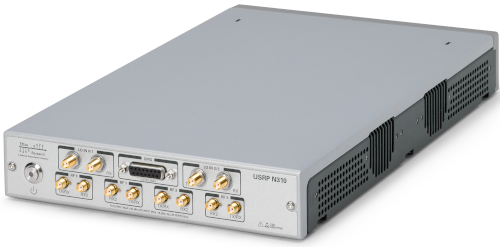
\includegraphics[width=1.5cm]{n310}} edge (matix);
  \node[right=.2cm of n310a, duplexer] (b77o) {n77} edge (n310a);
  \node[below right=-0.1cm and 0.35cm of b77o.east] (anto1)
    {
\includegraphics[width=0.3cm]{antenna}} edge (b77o);
  \node[above right=-0.1cm and 0.35cm of b77o.east] (anto2)
    {
\includegraphics[width=0.3cm]{antenna}} edge (b77o);

  \node[below right=-0.6cm and 2cm of porcepix, label=above:obelix] (obelix)
    {
\includegraphics[width=1.2cm]{server}}
    edge (porcepix);
  \node[right=0.3cm of obelix, label=above:N310] (n310o)
    {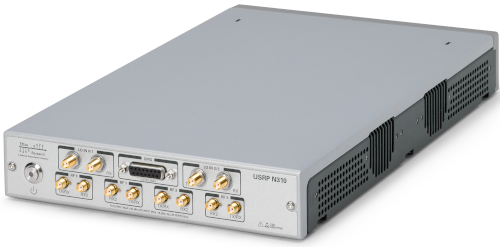
\includegraphics[width=1.5cm]{n310}} edge (obelix);
  \node[right=.2cm of n310o, duplexer] (b78o) {n40} edge (n310o);
  \node[below right=-0.1cm and 0.35cm of b78o.east] (anto1)
    {
\includegraphics[width=0.3cm]{antenna}} edge (b78o);
  \node[above right=-0.1cm and 0.35cm of b78o.east] (anto2)
    {
\includegraphics[width=0.3cm]{antenna}} edge (b78o);

  \node[below=2cm of porcepix, label=above:Cluster] (cluster)
    {
\includegraphics[width=1.2cm]{server}};
  \node[right=2cm of cluster, label=above:cacofonix] (cacofonix)
    {
\includegraphics[width=1.2cm]{server}}
      edge (cluster);
  \node[right=0.3cm of cacofonix, label=above:VVDN, draw,
        minimum width=1.7cm, minimum height=0.8cm] (vvdn)
    {O-RU} edge (cacofonix);
  \node[below right=+0.45cm and 0.35cm of vvdn.east] (antv1)
    {
\includegraphics[width=0.3cm]{antenna}} edge (vvdn.east);
  \node[below right=-0.1cm and 0.35cm of vvdn.east] (antv2)
    {
\includegraphics[width=0.3cm]{antenna}} edge (vvdn.east);
  \node[above right=-0.1cm and 0.35cm of vvdn.east] (antv3)
    {
\includegraphics[width=0.3cm]{antenna}} edge (vvdn.east);
  \node[above right=+0.45cm and 0.35cm of vvdn.east] (antv4)
    {
\includegraphics[width=0.3cm]{antenna}} edge (vvdn.east);

  \node[above right=+0.0cm and 5.0cm of n310o.east, label=above:RM520N-GL] (quectel)
    {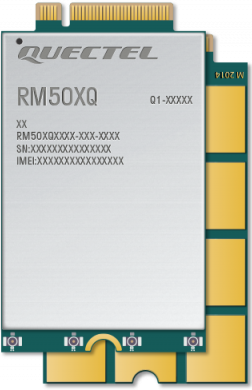
\includegraphics[height=1.2cm]{quectel}};
  \node[above left=-0.1cm and 0.8cm of quectel.west] (aq2)
    {
\includegraphics[width=0.3cm]{antenna}} edge (quectel);
  \node[above=-0.2cm of aq2] (aq1)
    {
\includegraphics[width=0.3cm]{antenna}} edge (quectel);
  \node[below=-0.2cm of aq2] (aq3)
    {
\includegraphics[width=0.3cm]{antenna}} edge (quectel);
  \node[below=-0.2cm of aq3]
    {
\includegraphics[width=0.3cm]{antenna}} edge (quectel);
  \node[right=1cm of quectel, label=above:up2] (up2)
    {
\includegraphics[width=1.2cm]{server}}
    edge (quectel);

\end{tikzpicture}
\end{document}
